% Level-set method comparison on the reversed 2D vortex. Compiles from day one;
% figures/tables are the single data source shared with comparison.template.html.
% Reproduce everything (runs + this PDF + the deck) with ONE command:
%   snakemake -s workflow/Snakefile.comparison --workflow-profile profiles/local
\documentclass[preprint,3p,11pt]{elsarticle}

\usepackage{amsmath,amssymb}
\usepackage{graphicx}
\usepackage{booktabs}

\graphicspath{{data/figures/}}

\newcommand{\psilev}{\psi}

\begin{document}
\begin{frontmatter}

\title{Which level-set advection method, given sufficient resolution?
A wall-clock-fair comparison on the reversed vortex}

\author[tuda]{Tomislav Mari\'{c}}
\author[tuda]{Mathis Fricke}
\author[tuda]{Dieter Bothe}
\address[tuda]{Mathematical Modeling and Analysis, TU Darmstadt, Germany}

\begin{abstract}
We compare four level-set advection strategies --- semi-Lagrangian
quadratic-reconstruction transport, defect-corrected Eulerian transport,
Eulerian transport with an SDPLS gradient-control source, and Eulerian
transport with interface-normal velocity extension --- on the reversed
single-vortex benchmark at resolutions from $32^2$ to $512^2$ and two
horizons $T \in \{2, 8\}$. All variants run through ONE dictionary-configured
solver at a fixed parallel decomposition ($n_p = 4$ everywhere), so the
reported wall-clock times are directly comparable. We measure shape error,
volume conservation and the signed-distance quality at the reversed state
$t = T$ and at maximal stretching $t = T/2$. Given sufficient resolution the
semi-Lagrangian quadratic method is the choice: at $512^2/T{=}8$ it is
$20\times$ more accurate than the best Eulerian variant at half the wall
clock, and its long-horizon accuracy matches its short-horizon accuracy once
the stretched filament is resolved. The SDPLS sources' one measurable
advantage --- volume conservation at maximal stretching --- is a coarse-mesh
effect that vanishes under refinement; velocity extension is dominated at
every resolution.
\end{abstract}

\begin{keyword}
level set \sep semi-Lagrangian \sep reinitialization \sep verification
\sep OpenFOAM
\end{keyword}
\end{frontmatter}

% ============================================================================
\section{The decision question}
Every level-set advection line in this code base (semi-Lagrangian,
velocity extension, SDPLS source, geometric redistancing) targets the same
problem: transport $\psilev$ accurately while keeping it usable as a signed
distance. The practical question for a user is not which line is most
elegant but which to \emph{choose} for a production run of given resolution
and cost budget. This note answers it with one benchmark.

% ============================================================================
\section{Setup}
\textbf{Case.} The reversed single (shear) vortex: a circle of radius $0.15$
in the unit square, advected by $\cos(\pi t/\tau)$-reversed shear so the
exact solution at $t = T$ is the initial circle. We sweep
$N \in \{32, 64, 128, 256, 512\}$ (cells per side) and $T \in \{2, 8\}$ at
$\mathrm{CFL} = 0.5$, with the geometric Detrixhe--Aslam phase indicator.

\textbf{Methods}, all through the unified \texttt{leiaLevelSetFoam} solver
(one \texttt{fvSolution.levelSet} dictionary selects the method):
semi-Lagrangian quadratic weighted least squares (cached and cache-free);
defect-corrected Eulerian transport in advective form; the same with an
SDPLS source (R and beta); and Eulerian transport with interface-normal
velocity extension (closest-point).

\textbf{Fair wall clock.} Every run uses the SAME parallel decomposition,
$n_p = 4$ MPI ranks, and the SAME reporting cadence (phase indicator and
error norms computed only at write times $\{0, T/2, T\}$), so the
\texttt{ELAPSED\_CLOCK\_TIME} totals compare method to method at each
$(N, T)$. (At fixed $n_p$ the per-rank load grows with $N$, so absolute
seconds mix solver cost with parallel efficiency; the method \emph{ranking}
at each $(N,T)$ is unaffected.)

\textbf{Metrics.} At $t = T$ (reversed state) we report the shape error
$E_{geom} = \sum_c V_c|\alpha_c - \alpha_c^0|$, the relative volume error,
and the band $L_2$ of $||\nabla\psilev|-1|$. At $t = T/2$ (maximal
stretching) the exact volume-fraction field of the stretched shape is
unknown, so we report only the volume conservation and the band gradient
error there.

% ============================================================================
\section{Results}
\subsection{Convergence}
Figure~\ref{fig:convT2} (T = 2, resolved) and Figure~\ref{fig:convT8}
(T = 8, filament) show the five metrics per method over $h$. Individual
enlarged panels are in \texttt{data/figures/benchVortex\_T\{2,8\}\_*.png}.

\begin{figure}[htbp]
  \centering
  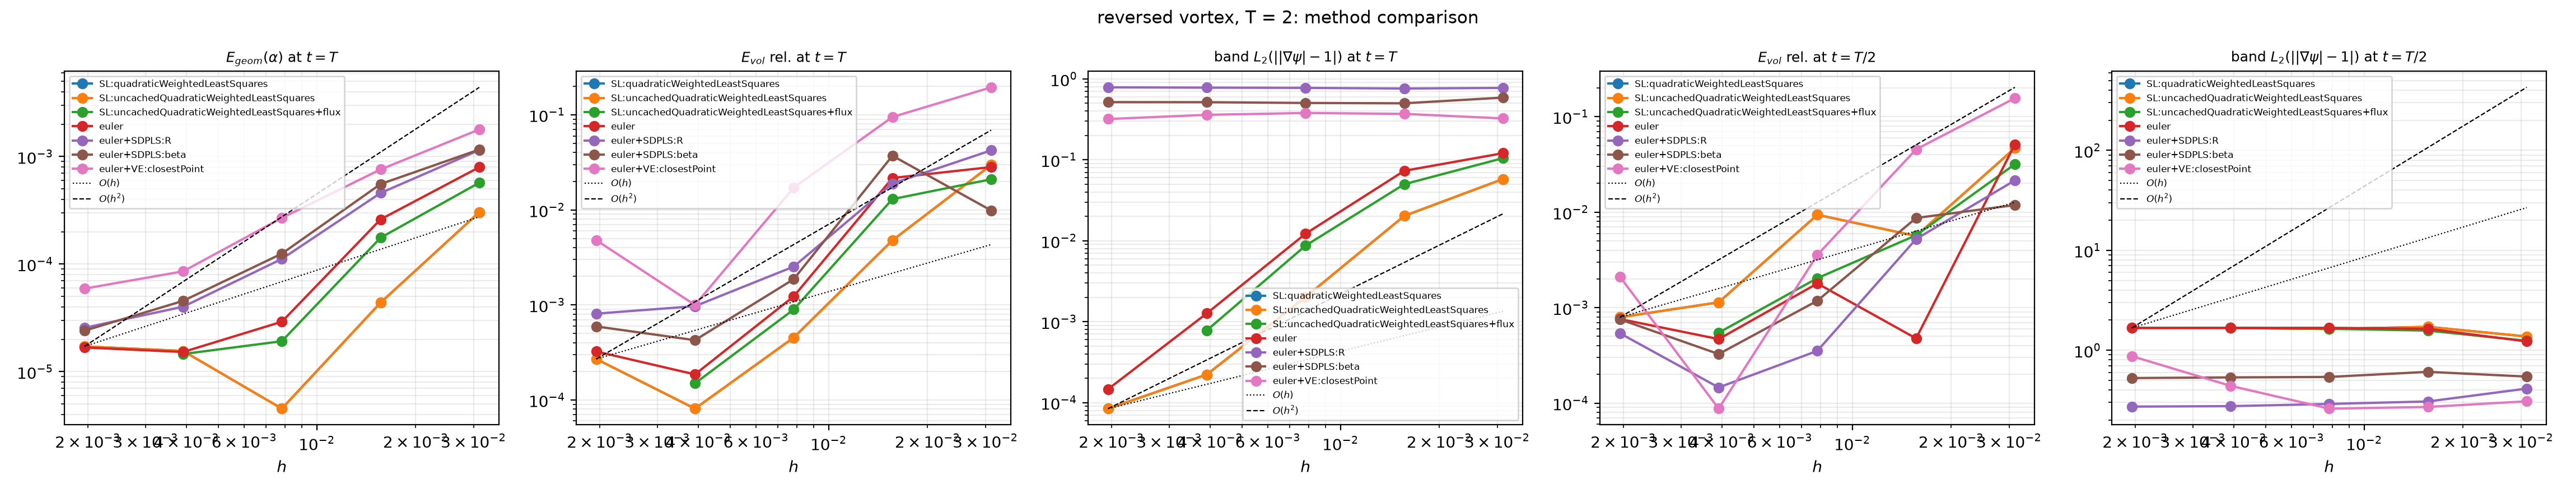
\includegraphics[width=\linewidth]{benchVortex_convergence_T2.png}
  \caption{Convergence at $T = 2$ (resolved regime). Shape / volume / band
    gradient at $t = T$; volume + band gradient at $t = T/2$.}
  \label{fig:convT2}
\end{figure}

\begin{figure}[htbp]
  \centering
  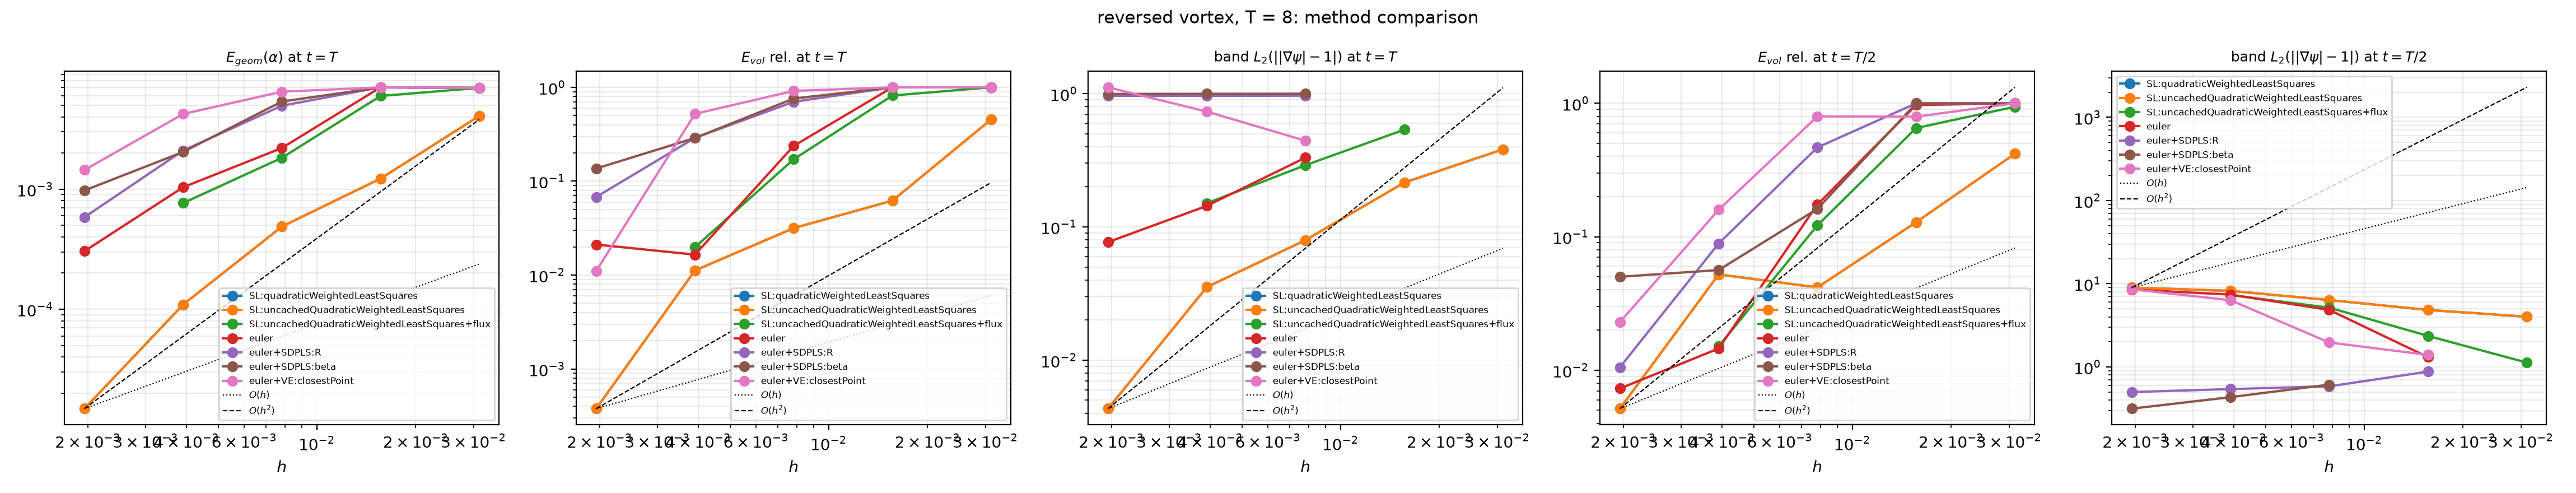
\includegraphics[width=\linewidth]{benchVortex_convergence_T8.png}
  \caption{Convergence at $T = 8$ (filament regime). At $N \le 128$ the
    stretched filament is under-resolved for every method; $256^2/512^2$
    restore the $T = 2$ ranking.}
  \label{fig:convT8}
\end{figure}

\subsection{Cost versus accuracy}
\begin{figure}[htbp]
  \centering
  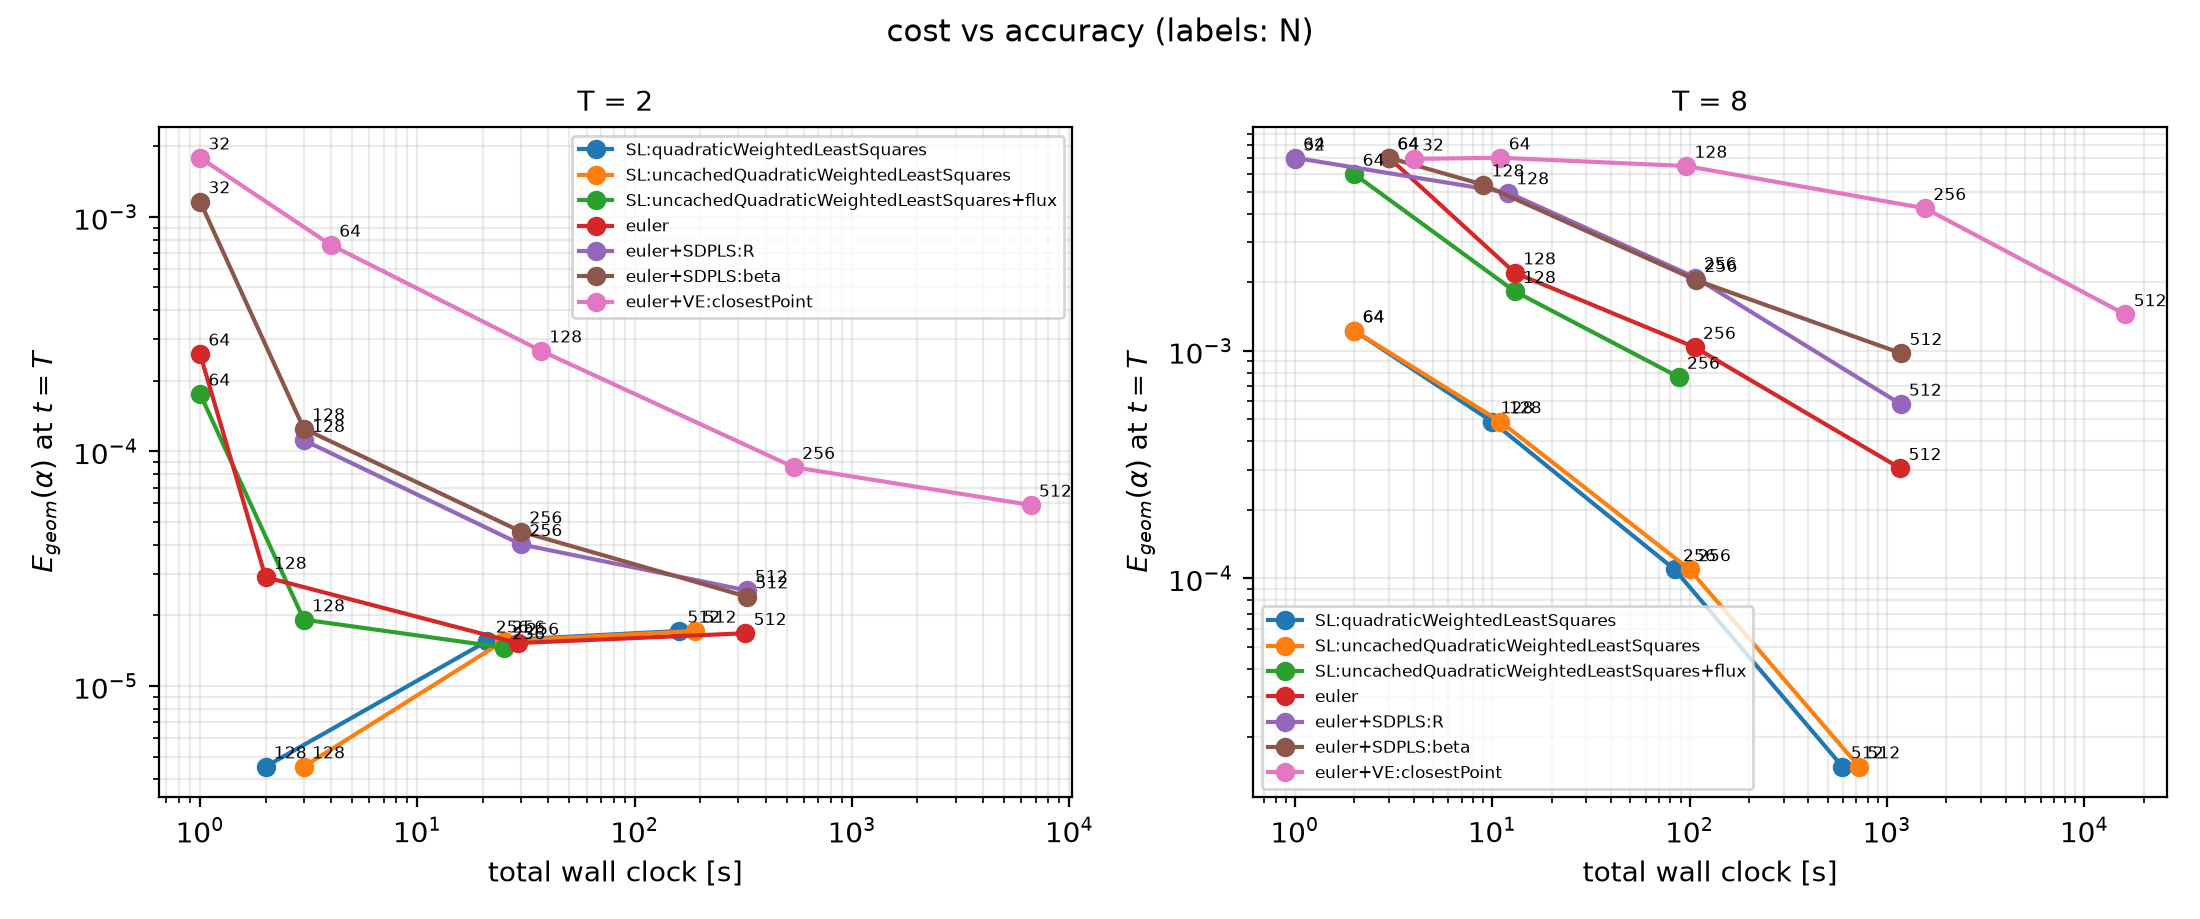
\includegraphics[width=\linewidth]{benchVortex_cost_accuracy.png}
  \caption{Total wall clock (s, $n_p = 4$) versus shape error at $t = T$;
    point labels are $N$. Down-left is better.}
  \label{fig:cost}
\end{figure}

\subsection{The decision table}
Table~\ref{tab:decision} lists, per method and horizon, the finest-mesh
errors and the total wall clock.
\begin{table}[htbp]
  \centering
  \caption{Finest-mesh ($N = 512$) errors and wall clock per method.}
  \label{tab:decision}
  \resizebox{\linewidth}{!}{\begin{tabular}{l l r r r r r r}
\hline
method & $T$ & $N$ & $E_{geom}$ & $E_{vol}$ & band grad & $E_{vol}^{T/2}$ & clock [s] \\
\hline
SL:quadraticWeightedLeastSquares & 2 & 512 & 1.72e-05 & 2.70e-04 & 8.41e-05 & 7.92e-04 & 1.60e+02 \\
SL:uncachedQuadraticWeightedLeastSquares & 2 & 512 & 1.72e-05 & 2.70e-04 & 8.41e-05 & 7.92e-04 & 1.90e+02 \\
SL:uncachedQuadraticWeightedLeastSquares+flux & 2 & 256 & 1.46e-05 & 1.49e-04 & 7.80e-04 & 5.46e-04 & 2.50e+01 \\
euler & 2 & 512 & 1.68e-05 & 3.24e-04 & 1.46e-04 & 7.60e-04 & 3.23e+02 \\
euler+SDPLS:R & 2 & 512 & 2.56e-05 & 8.09e-04 & 7.87e-01 & 5.39e-04 & 3.27e+02 \\
euler+SDPLS:beta & 2 & 512 & 2.40e-05 & 5.93e-04 & 5.16e-01 & 7.54e-04 & 3.29e+02 \\
euler+VE:closestPoint & 2 & 512 & 5.91e-05 & 4.80e-03 & 3.19e-01 & 2.11e-03 & 6.63e+03 \\
\hline
SL:quadraticWeightedLeastSquares & 8 & 512 & 1.49e-05 & 3.77e-04 & 4.33e-03 & 5.15e-03 & 5.95e+02 \\
SL:uncachedQuadraticWeightedLeastSquares & 8 & 512 & 1.49e-05 & 3.77e-04 & 4.33e-03 & 5.15e-03 & 7.22e+02 \\
SL:uncachedQuadraticWeightedLeastSquares+flux & 8 & 256 & 7.66e-04 & 1.98e-02 & 1.50e-01 & 1.51e-02 & 8.80e+01 \\
euler & 8 & 512 & 3.04e-04 & 2.11e-02 & 7.69e-02 & 7.29e-03 & 1.17e+03 \\
euler+SDPLS:R & 8 & 512 & 5.83e-04 & 6.79e-02 & 9.62e-01 & 1.05e-02 & 1.17e+03 \\
euler+SDPLS:beta & 8 & 512 & 9.75e-04 & 1.36e-01 & 9.94e-01 & 5.01e-02 & 1.18e+03 \\
euler+VE:closestPoint & 8 & 512 & 1.44e-03 & 1.11e-02 & 1.11e+00 & 2.29e-02 & 1.61e+04 \\
\hline
\end{tabular}
}
\end{table}

\subsection{Detailed comparison (all methods)}
Table~\ref{tab:detailed} lists every method line and variant at its finest
resolution, with the least-squares convergence orders $p_{geom}$, $p_{vol}$
over the swept mesh sequence.
\begin{table}[htbp]
  \centering
  \caption{All methods, finest $N$: errors, convergence orders, wall clock.
    Core method lines run to $512^2$; the SL-improvement and redistancing
    variants to $256^2$.}
  \label{tab:detailed}
  \resizebox{\linewidth}{!}{\begin{tabular}{l c c c c c c c}
\hline
method & $T$ & $N$ & $E_{geom}$ & $p_{geom}$ & $E_{vol}$ & $p_{vol}$ & clock [s] \\
\hline
SL quad (cached) & 2 & 512 & 1.72e-05 & -0.98 & 2.70e-04 & -1.94 & 160.00 \\
SL quad (uncached) & 2 & 512 & 1.72e-05 & -0.98 & 2.70e-04 & -1.94 & 190.00 \\
SL quad (uncached) + flux-form & 2 & 256 & 1.46e-05 & -1.91 & 1.49e-04 & -2.53 & 25.00 \\
euler & 2 & 512 & 1.68e-05 & -1.52 & 3.24e-04 & -1.98 & 323.00 \\
euler + SDPLS:R & 2 & 512 & 2.56e-05 & -1.45 & 8.09e-04 & -1.57 & 327.00 \\
euler + SDPLS:beta & 2 & 512 & 2.40e-05 & -1.48 & 5.93e-04 & -1.46 & 329.00 \\
euler + VE:closestPoint & 2 & 512 & 5.91e-05 & -1.30 & 4.80e-03 & -1.73 & 6630.00 \\
SL quad (uncached) + venk & 2 & 256 & 3.74e-05 & -1.02 & 2.48e-03 & 0.54 & 30.00 \\
SL quad (uncached) + QR [pert mesh] & 2 & 128 & 6.44e-05 & -1.07 & 4.08e-04 & -3.07 & 3.00 \\
SL quad (uncached) [pert mesh] & 2 & 128 & 6.44e-05 & -1.07 & 4.08e-04 & -3.07 & 2.00 \\
SL quad (cached) & 8 & 512 & 1.49e-05 & -1.97 & 3.77e-04 & -2.29 & 595.00 \\
SL quad (uncached) & 8 & 512 & 1.49e-05 & -1.97 & 3.77e-04 & -2.29 & 722.00 \\
SL quad (uncached) + flux-form & 8 & 256 & 7.66e-04 & -1.13 & 1.98e-02 & -1.92 & 88.00 \\
euler & 8 & 512 & 3.04e-04 & -1.18 & 2.11e-02 & -1.70 & 1167.00 \\
euler + SDPLS:R & 8 & 512 & 5.83e-04 & -0.89 & 6.79e-02 & -0.95 & 1171.00 \\
euler + SDPLS:beta & 8 & 512 & 9.75e-04 & -0.75 & 1.36e-01 & -0.75 & 1179.00 \\
euler + VE:closestPoint & 8 & 512 & 1.44e-03 & -0.53 & 1.11e-02 & -1.39 & 16131.00 \\
SL quad (uncached) + venk & 8 & 256 & 4.45e-04 & -1.15 & 4.94e-02 & -1.03 & 101.00 \\
euler + frozen-redist & 8 & 256 & 1.33e-02 & 0.24 & 1.77e+00 & 2.15 & 1259.00 \\
\hline
\end{tabular}
}
\end{table}

\subsection{Where the flux-form volume loss comes from}
\label{sec:fluxloss}
Time-resolving the reversed vortex at $N = 128$ isolates the mechanism
(Figure~\ref{fig:fluxloss}). At $T = 2$ the flux-form and point-value schemes
are indistinguishable: the band gradient histories coincide and the final
volume error is $0.06\%$. The difference appears only at $T = 8$, and it is
\emph{numerical dissipation from the upwind finite-volume flux}. The flux
evaluates the upwind cell's reconstruction at the face --- a dissipative,
irreversible operation. When the reversed vortex compresses the interface toward
sub-cell scale (the band mean $|\nabla\psi|$ climbs to ${\approx}5$), that
dissipation smears the steepened $\psi$: the flux-form volume drops
\emph{monotonically} ($-17\%$ by $t = 6.5$) because dissipation cannot be
undone, whereas the point-value SL --- a pure characteristic interpolation with
no dissipation --- only oscillates ($\pm1\%$) and \emph{recovers} on flow
reversal, its errors being dispersive and hence reversible. The flux-form ends
with band $|\nabla\psi| = 0.72 < 1$ (a flattened, eroded interface) against
point-value's $0.96$. Throughout, $\int\psi\,dV$ stays conserved to machine
precision --- the dissipation redistributes $\psi$ conservatively --- but since
$\alpha = H(-\psi)$ is a nonlinear functional, a smeared $\psi$ places the zero
contour inside the true interface, and the phase volume is lost.
\begin{figure}[htbp]
  \centering
  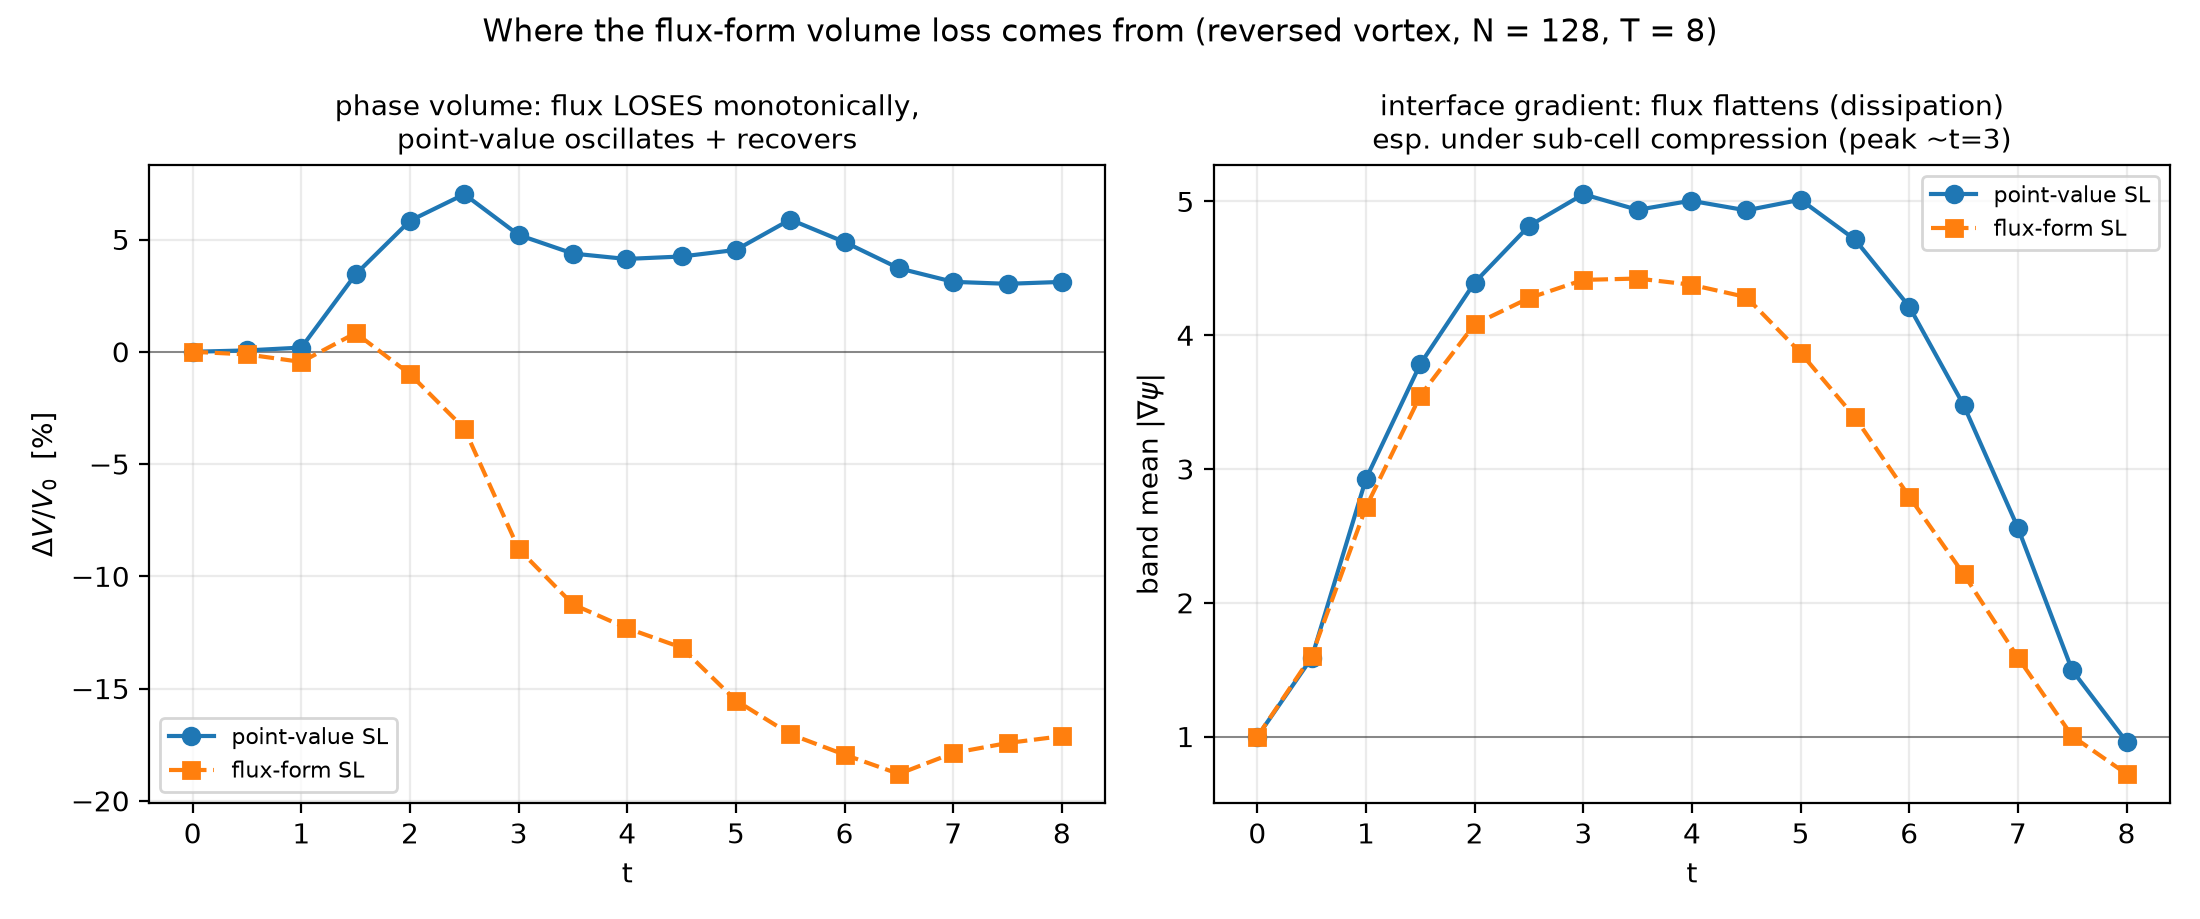
\includegraphics[width=\linewidth]{benchVortex_fluxvolloss.png}
  \caption{Reversed vortex, $N = 128$, $T = 8$. Left: relative phase volume ---
    flux-form loses monotonically (irreversible dissipation), point-value
    oscillates and recovers. Right: band $|\nabla\psi|$ --- flux-form flattens
    below one under sub-cell compression.}
  \label{fig:fluxloss}
\end{figure}

\subsection{Field atlas}
Figure~\ref{fig:atlas} contrasts the semi-Lagrangian winner with the
Eulerian baseline at $T = 8$: the volume fraction (top) and the
signed-distance quality (bottom) across resolutions. The full atlas (every
method $\times$ $\{\alpha, \psilev, ||\nabla\psilev|-1|\}$ $\times$ $T$) is
in \texttt{data/figures/bench\_*.png}.
\begin{figure}[htbp]
  \centering
  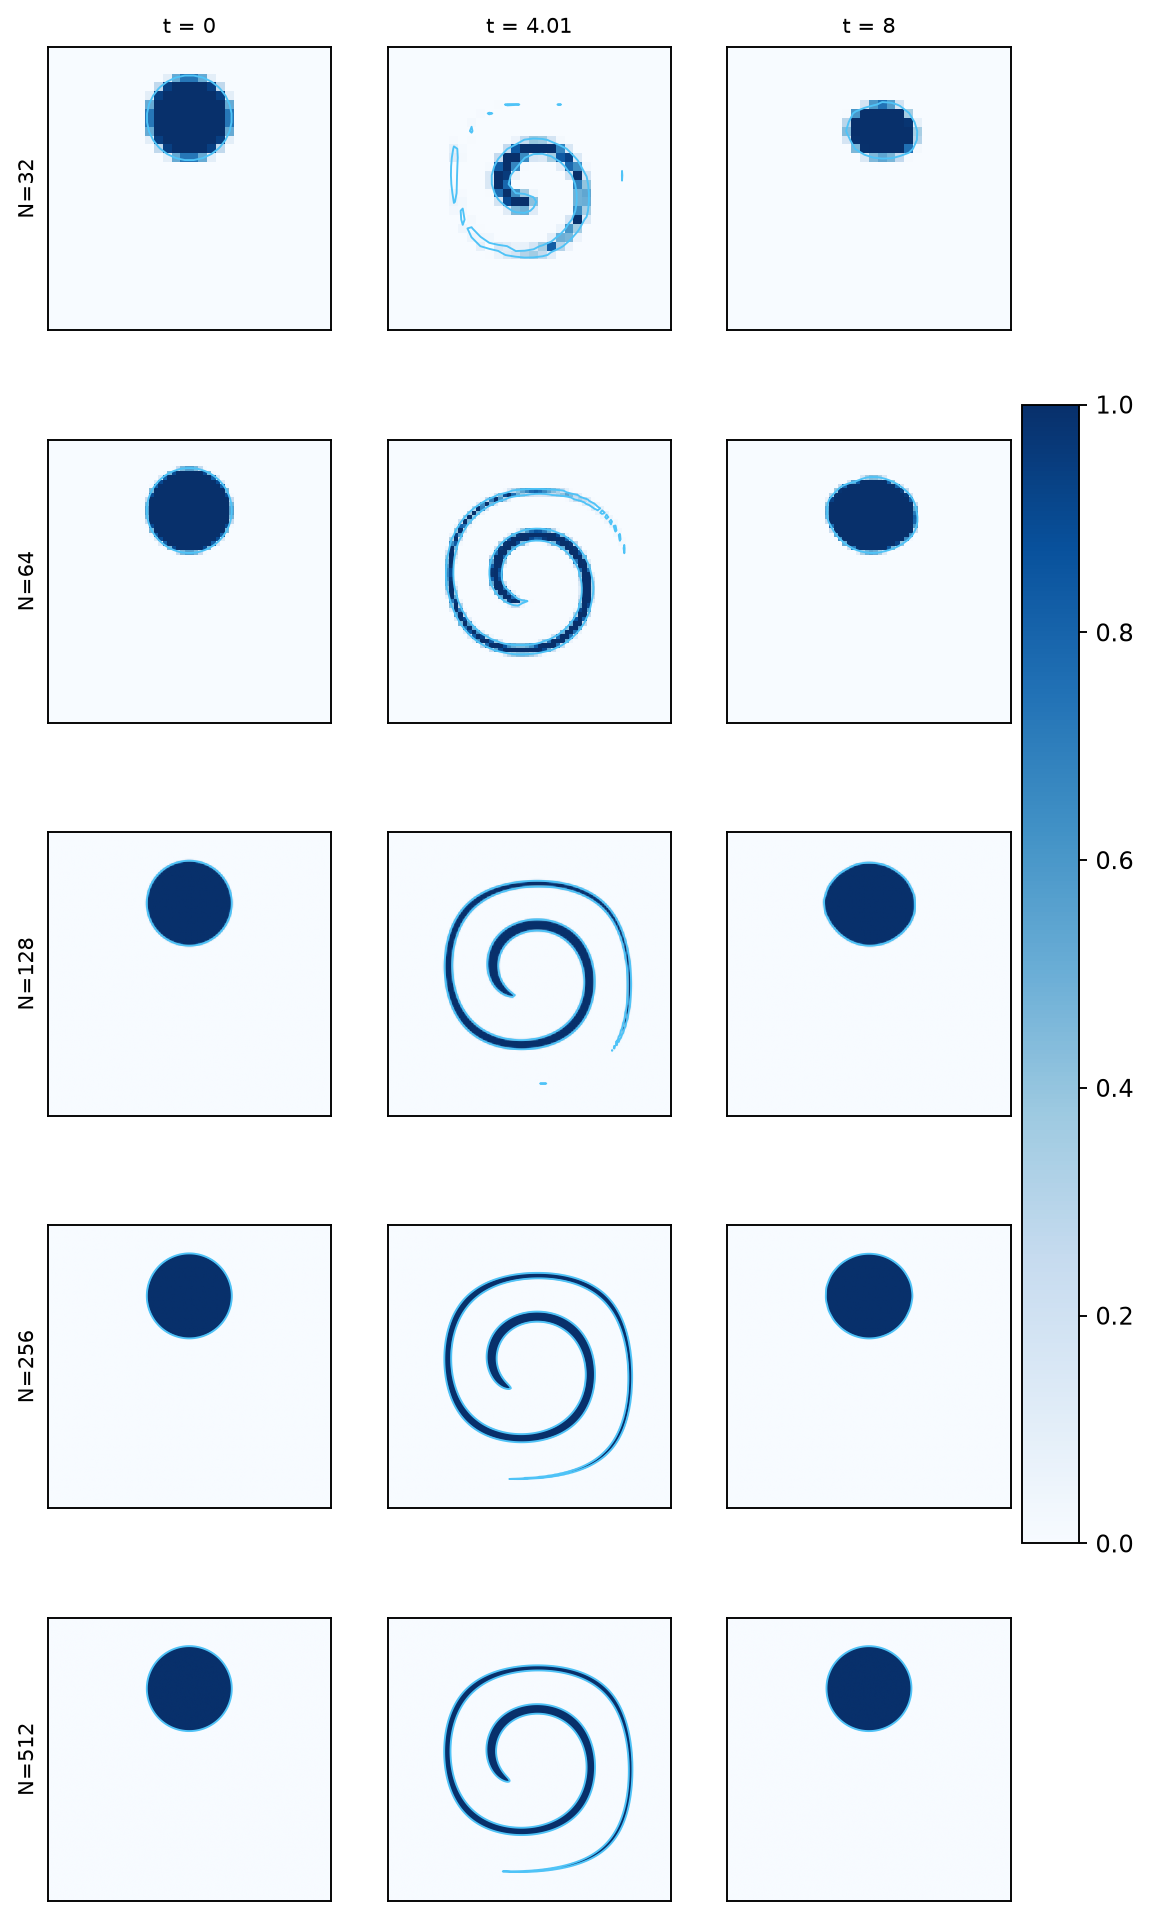
\includegraphics[width=0.49\linewidth]{bench_SL_quadraticWeightedLeastSquares_T8_alpha.png}
  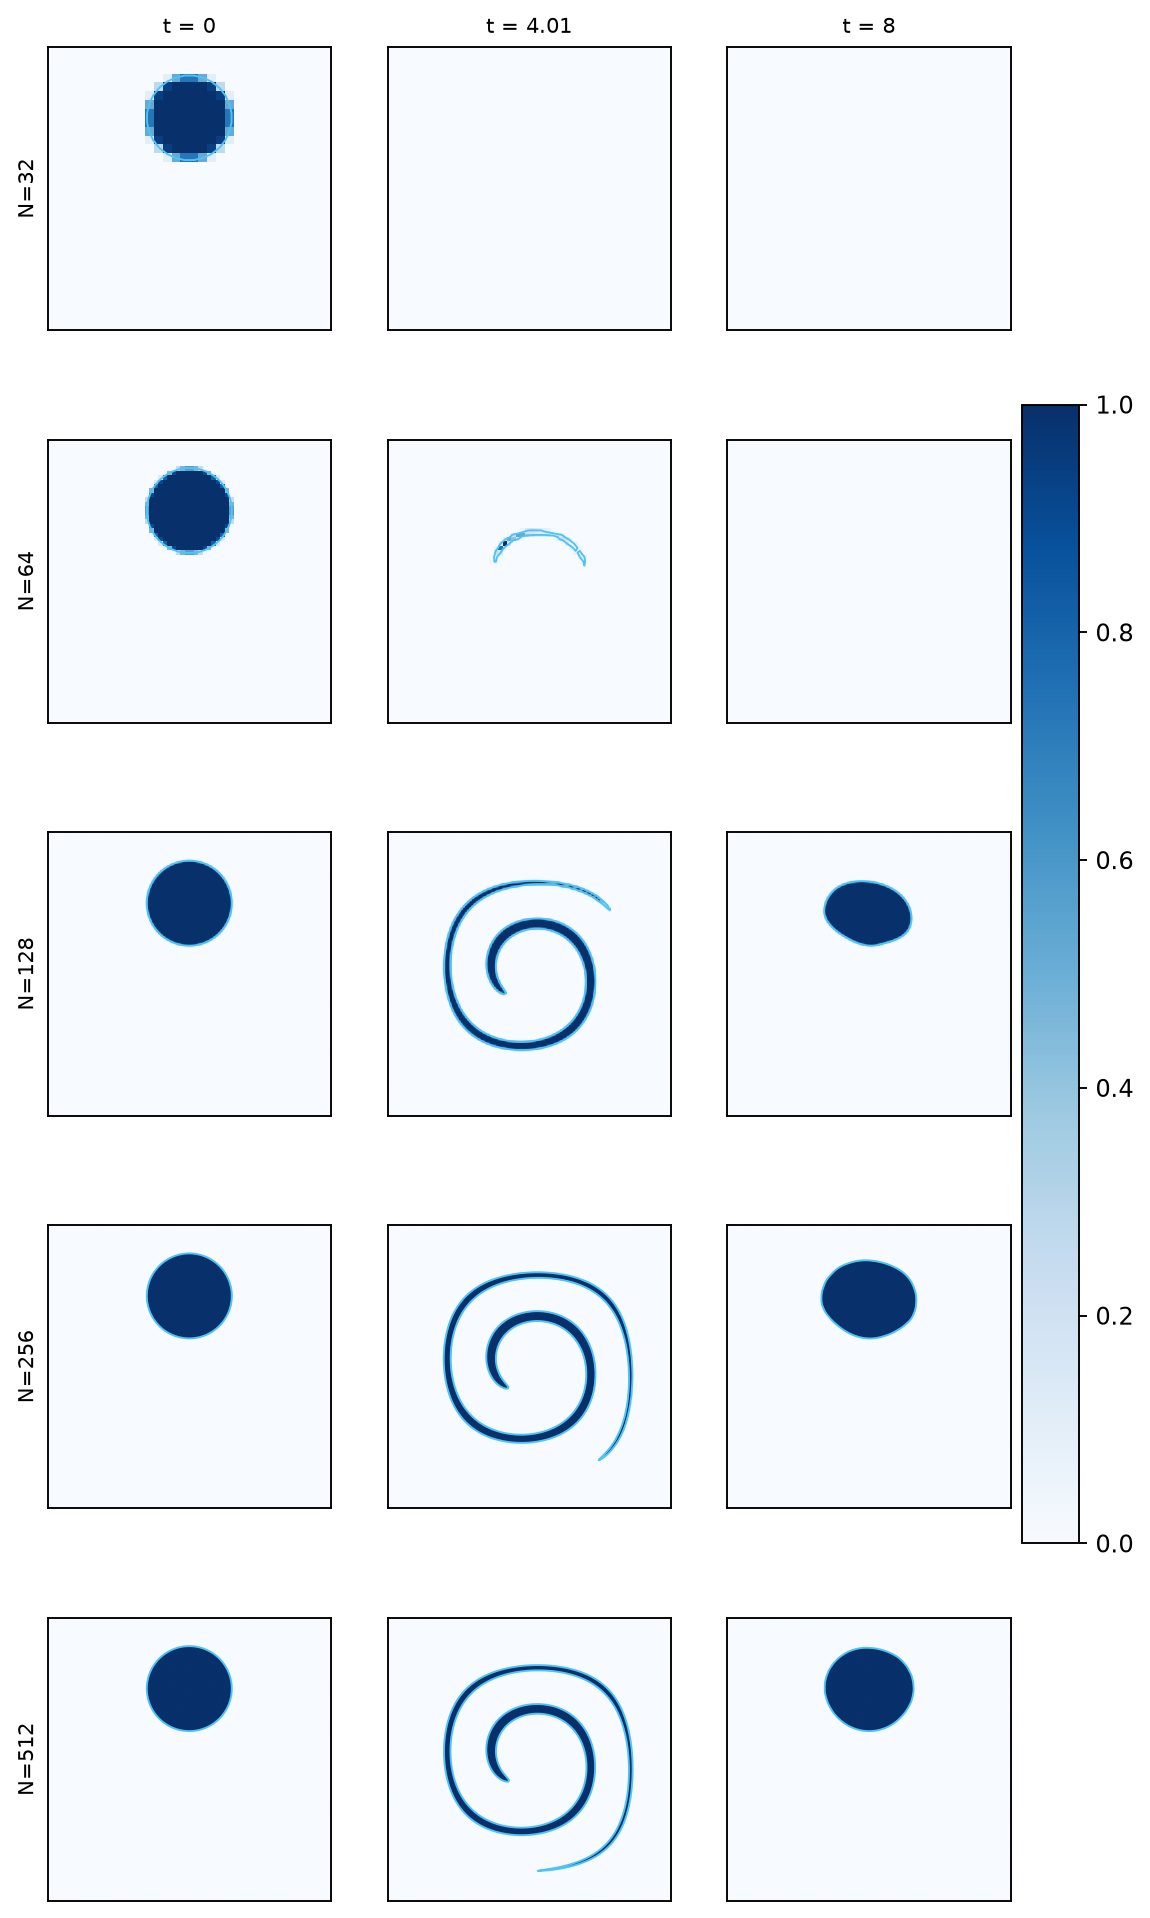
\includegraphics[width=0.49\linewidth]{bench_euler_T8_alpha.png}
  \caption{$\alpha$ at $T = 8$: semi-Lagrangian (left) vs.\ Eulerian
    (right); rows are $N$, columns $t \in \{0, T/2, T\}$, cyan is the zero
    level set.}
  \label{fig:atlas}
\end{figure}

% ============================================================================
\section{Verdict}
Given sufficient resolution, choose semi-Lagrangian quadratic transport: it
is the most accurate AND the cheapest method at every measured resolution
and horizon (at $512^2/T{=}8$, $20\times$ the accuracy of the best Eulerian
at half the wall clock, $27\times$ cheaper than velocity extension), and its
$T = 8$ accuracy equals its $T = 2$ accuracy once the filament is resolved.
Plain defect-corrected Eulerian transport is a robust second. The SDPLS
sources earn their place for volume conservation under maximal stretching on
coarse meshes and for two-phase coupling (zero interface displacement), not
for end-state accuracy in pure advection. Velocity extension is dominated.
The under-resolution death of the $T = 8$ filament at $N \le 64$ is
method-independent --- refinement, not gradient maintenance, is the cure.

% ============================================================================
\section{Limitations and outlook}
Each method's dominant fault (code-documented or benchmark-measured) and its
most promising fix:
\begin{description}
  \item[Semi-Lagrangian quadratic] No maximum principle -- quadratic fits
    overshoot, and a hard Barth--Jespersen limiter collapses the convergence
    order ($3.0\to0.1$). Improvements implemented here: an order-preserving
    Venkatakrishnan limiter, a Householder-QR least-squares solve (no
    condition-number squaring), and a conservative flux-form variant that
    conserves $\int\psi\,dV$ to machine precision (Section~\ref{sec:slimp}).
    Outstanding: the cached model's memory ceiling in 3D and a
    genuinely mass-conserving phase volume.
  \item[Eulerian defect-corrected PDE] linearUpwind numerical diffusion erodes
    $|\nabla\psi|$ and the deferred correction costs $2$--$3$ assembles per
    step; $20\times$ behind SL at $512^2/T{=}8$. A higher-order bounded flux
    (WENO / limited-cubic) would cut the diffusion without the defect-correction
    cost.
  \item[SDPLS source] Trades the signed-distance property for gradient control
    and over-flattens near the resolution limit ($R$: volume error $0.49$ vs
    $0.24$ without a source at $T{=}8$, $N{=}128$); $\beta$ with an explicit
    discretization diverges at every CFL. A resolution-aware ($\kappa h$)
    gating of the source, and an always-implicit $\beta$, are the fixes; its
    niche is two-phase coupling (zero interface displacement), not pure
    advection.
  \item[Velocity extension] Dominated: worst accuracy at $12$--$27\times$ the
    cost, the per-step extension solve being the overhead, with geometric
    failure modes (colliding rays, a circular dependency on redistancing).
    Restrict it to problems that genuinely need an extended velocity (moving
    contact lines); replace the solve with a cheap geometric (fast-marching)
    extension otherwise.
  \item[Geometric redistancing (retired, one survivor)] The zero level set
    and the band values are the same degrees of freedom, so any band rewrite
    displaces the interface ($\mathcal{O}(h^2\kappa)$ per event, compounding).
    Superseded by the SDPLS source for $\psi$-maintenance. The one surviving
    configuration is implemented and gated: \emph{frozen-band bulk-only}
    pseudo-time Eikonal redistancing --- the sign-change band plus two guard
    layers keep their \emph{transported} values as Dirichlet anchors (nothing
    is reconstructed, so no chord bias; one static event gives $E_{geom} =
    E_{vol} = 0$ exactly and bitwise-unchanged anchors), and the bulk is
    re-extended with a Godunov (Rouy--Tourin) upwind Hamiltonian (bulk
    gradient error $0.56 \to 0.009$ per event, where the central-gradient
    operator diverges $0.56 \to 59.7$ and flips bulk signs). Its measured
    transport verdict is in Section~\ref{sec:frozen}.
  \item[Phase indicator (shared)] The least-squares plane is a chord of the
    curved interface, an $\mathcal{O}(h^2\kappa)$ one-signed bias that caps
    $\alpha$ at second order. A curvature-corrected plane distance (the
    chord-bias subtraction already used in the redistancer anchors), or a
    PLIC/ELVIRA reconstruction, would lift the order.
\end{description}

\subsection{Measured semi-Lagrangian improvements (mostly negative)}
\label{sec:slimp}
The three implemented SL improvements were re-tested on the reversed vortex
(\texttt{config/benchVortexSLimproved}, \texttt{...Perturbed}, \texttt{...flux});
the honest outcome is that only one of the three earns its keep unconditionally.

\textbf{Venkatakrishnan limiter} ($K = 5$): the shape-error convergence order
drops from $\approx 3.0$ (unlimited) to $\approx 0.9$ --- far better than the
Barth--Jespersen stall at $0.1$, but not order-preserving in the advection
setting; $L_\infty(e_\psi)$ worsens at every $N$ except $32$. Its wins are
coarse-mesh volume conservation ($N{=}32$, $T{=}2$: $2.97\times10^{-2} \to
7.4\times10^{-4}$) and band-gradient control ($0.98 \to 0.74$). Moreover the
boundedness metric it targets was already zero: the geometric phase indicator
bounds $\alpha$ by construction. Verdict: keep it off on hex meshes; it is the
softer alternative to the hard stencil clamp where polyhedral overshoot demands
a guard.

\textbf{Householder-QR least squares}: bit-parity with the Cholesky normal
equations on hex \emph{and} on an $\alpha{=}0.1$-perturbed mesh (errors
identical to the last digit, zero degenerate fallbacks in either) --- free
robustness. The ill-conditioning it guards against (near-coplanar stencils)
was not reachable in these 2D studies; it remains the safeguard for
polyhedral/CFC stencils.

\textbf{Flux-form (conservative) SL}: a distinct conservative advection scheme
(its own RTS \texttt{slScheme}) that conserves $\int\psi\,dV$ to
$2\times10^{-14}$. At the resolved horizon ($T = 2$) it is \emph{competitive}
with point-value transport --- the same convergence order (${\approx}2.5$--$3$
on volume, ${\approx}2$--$3$ on shape) with errors within ${\approx}2\times$,
and at the finest mesh ($256^2$) its shape error ($1.5\times10^{-5}$) edges
point-value, whose shape error stalled from $128^2$ to $256^2$. Its one cost is
the extra numerical diffusion of the half-step swept-flux evaluation, a roughly
constant factor when the interface is resolved that compounds only on the
extreme long horizon: at $T = 8$, over eight revolutions of a sub-cell filament,
its volume error is $3$--$13\times$ that of point-value ($N{=}64$: $0.82$ vs
$0.062$). Verdict: an attractive conservative alternative when the interface is
resolved and $\int\psi$ conservation is wanted; point-value remains the choice
for extreme long-horizon thin-filament transport.

A pitfall surfaced on the way: \texttt{leiaPerturbMesh} was a no-op on 2D
meshes (every point of a one-cell-thick mesh lies on the empty patches, and
the boundary reset silently reverted the entire perturbation); it is fixed
(only physical patches pinned, empty-direction component zeroed, deterministic
seed), and the perturbed study is the first to actually run on a perturbed
mesh.

\subsection{Frozen-band redistancing: the last redistancing candidate, measured}
\label{sec:frozen}
The frozen-band bulk-only redistancer was engineered to evade every measured
reason the geometric-redistancing line was retired: its Dirichlet anchors make
one static event provably zero-displacement ($E_{geom} = E_{vol} = 0$, anchors
bitwise unchanged), and the Godunov Hamiltonian cures the central operator's
divergence. Coupled to Eulerian transport over a $T = 8$ reversed vortex
(\texttt{config/benchVortexGRLfrozen}), it nonetheless \emph{injures} the
simulation. Against no redistancing, at the two resolved resolutions the volume
error inflates by one to two orders of magnitude:

\begin{center}
\begin{tabular}{lccc}
\toprule
$N$ & no redistancing $E_{vol}$ & frozen-band $E_{vol}$ & frozen-band $E_{geom}$ \\
\midrule
256 & 0.017 & 1.77 & 0.013 \\
128 & 0.238 & 2.53 & 0.021 \\
 64 & 1.0 (filament dead) & 0.090 & 0.010 \\
\bottomrule
\end{tabular}
\end{center}

The mechanism is the fundamental redistancing lesson made precise: a redistancer
faithfully rebuilds a signed distance to \emph{whatever} zero level set the
input field carries. Eulerian linearUpwind advection produces bounded but
nonzero over- and undershoots in the bulk --- spurious sign changes far from the
true interface. The frozen anchors freeze the true band correctly (hence the
static gate passes), but the bulk fill then reconstructs distance to those
spurious bulk zero-crossings, and the geometric indicator reads them as phase
(measured $\int\alpha$ inflated to $2.8\times$ the droplet at $N = 256$).
Redistancing cannot distinguish the interface from transport noise; it entrenches
the noise. This closes the line: even the configuration with provably zero
interface displacement injures the coupled run, because the injury does not come
from moving the interface --- it comes from rebuilding distance to advection
artefacts. The SDPLS source remains the sole viable $\psi$-maintenance mechanism
precisely because it never touches the sign structure (a smooth source vanishing
on the zero set cannot manufacture an interface).

% ============================================================================
\section{Reproducibility}
Everything in this note --- all runs, this PDF, and the companion reveal
deck --- regenerates with one command:
\begin{verbatim}
snakemake -s workflow/Snakefile.comparison --workflow-profile profiles/local
\end{verbatim}
which runs the six \texttt{config/benchVortex*.yaml} studies, harvests the
figures and the decision table into \texttt{data/}, rebuilds the deck, and
compiles this article.

\end{document}
